\documentclass[aspectratio=169, handout]{beamer}
%%%%%%%%%%%%%%%%%%%%%%%
% Packages %%%%%%%%%%%%
%%%%%%%%%%%%%%%%%%%%%%%
\usepackage{graphicx, hyperref, tikz, pgfplots, subfiles}
\usepackage[style = authoryear,maxcitenames = 2, hyperref=false]{biblatex}\addbibresource{references.bib}
\pgfplotsset{compat=1.18}    %     (any recent version is fine)
\usetikzlibrary{positioning, fit, backgrounds, patterns}
%\makeatletter
%\makeatother


%%%%%%%%%%%%%%%%%%%%%%%
% Defining Objects %%%%
%%%%%%%%%%%%%%%%%%%%%%%
\newcommand{\bparam}{b}
\newcommand{\cparam}{c}

%%%%%%%%%%%%%%%%%%%%%%%
% Head %%%%%%%%%%%%%%%%
%%%%%%%%%%%%%%%%%%%%%%%
\title{Commitment Can be Bad}
\author{Maximilian Reith}
\institute{University of Oxford}
\usepackage{Chapters_slides/SimplePlus}
\usepackage{graphicx, tikz, pgfplots, subfiles}
\usepackage[
    style=authoryear-icomp,
    maxcitenames=2,
    mincitenames=1,
    backend=biber,
    uniquelist=false
]{biblatex}
\pgfplotsset{compat=1.18}    %     (any recent version is fine)
\usetikzlibrary{positioning, fit, backgrounds, patterns}



\begin{document}

\begin{frame}{AI Game Theory}
\centering
\textit{Agents with different properties, games with different outcomes?}
\pause

\vspace{1em} % <-- adjust spacing here

\raggedright
Different properties could include \pause
\begin{itemize}
    \item Simulatability  \parencite{cooper_characterising_2024, kovarik_game_2024}\pause
    \item Imperfect Recall  \parencite{chen_imperfect_2024}\pause
    \item Greater Computational Capacity \pause
    \item Copyability \pause
    \item Ability to Commit \pause
    \item Modifiable Preferences
\end{itemize}
\end{frame}

\begin{frame}{Commitment}
\pause
\begin{itemize}
    \item It's easy to see how commitment could lead to more cooperation. \pause
    \item But can commitment be used as a threat? And lead to more conflict? \parencite[]{kokotajlo_commitment_2019}
\end{itemize}


\end{frame}
\begin{frame}{Game of Chicken}
\pause
\centering
\renewcommand{\arraystretch}{1.2}
\begin{tabular}{c|cc}
           & \textbf{Straight} & \textbf{Move} \\ \hline
\textbf{Straight} & $-1,\,-1$ & $\;\;1,\,-\tfrac12$ \\[2pt]
\textbf{Move}   & $-\tfrac12,\,1$ & $\;\;0,\,0$
\end{tabular}
\medskip
\pause
\begin{itemize}
  \item Two pure Nash equilibria (off-diagonal)
  \item Mixed equilibrium: Straight w.p.\ $2/3$
\end{itemize}
\end{frame}
\begin{frame}{Game of Chicken with Commitment}
\pause
    \begin{figure}[ht]
    \centering
    \resizebox{0.8\textwidth}{!}{%
        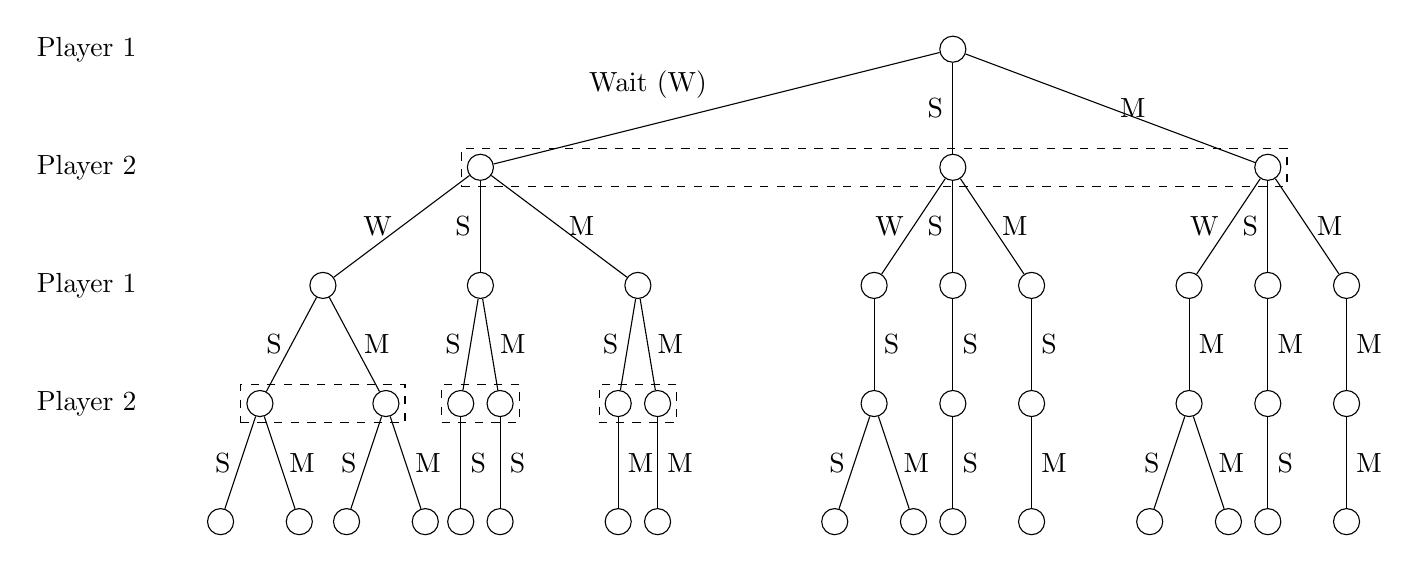
\begin{tikzpicture}
        %--- Macros with Updated Labels ---
        \newcommand{\firststage}[2]{%
            % Nodes for Player 2 at period 1 (following Player 1's move)
            \node (#11) [circle, draw, below of=#1, xshift=-#2, yshift=\yshift]{};
            \node (#12) [circle, draw, below of=#1, xshift=0, yshift=\yshift]{};
            \node (#13) [circle, draw, below of=#1, xshift=#2, yshift=\yshift]{};
            % Branches: left branch is Wait (W); the others are S and M.
            \draw (#1) -- (#11) node[midway, left] {W};
            \draw (#1) -- (#12) node[midway, left] {S};
            \draw (#1) -- (#13) node[midway, right] {M};
        }
        
        \newcommand{\aftercommit}[2]{%
            % Node following a committed action (only one possible continuation)
            \node (#11) [circle, draw, below of=#1, xshift=0, yshift=\yshift]{};
            \draw (#1) -- (#11) node[midway, right] {#2};
        }
        
        \newcommand{\afternocommit}[4]{%
            % Node for the noncommitted branch (with two possible moves)
            \node (#11) [circle, draw, below of=#1, xshift=-#2, yshift=\yshift]{};
            \node (#12) [circle, draw, below of=#1, xshift=#2, yshift=\yshift]{};
            \draw (#1) -- (#11) node[midway, left] {#3};
            \draw (#1) -- (#12) node[midway, right] {#4};
        }
        
        %--- Define Shift Variables ---
        \newcommand{\xshiftA}{5cm}           % For first stage    
        \newcommand{\xshiftfollowone}{0.25cm}  % For third stage (single branch)
        \newcommand{\xshiftC}{0.5cm}          % For fourth stage
        \newcommand{\xshiftlabel}{-10cm}      % For labels
        \newcommand{\yshift}{-0.5cm}
        
        %--- Root Node (Player 1) ---
        \node (root) at (0,0) [circle, draw] {};
        
        % Player 1’s initial decision: Wait, commit to S, or commit to M
        \node (child1) [circle, draw, below of=root, xshift=-\xshiftA-1cm, yshift=\yshift]{};
        \node (child2) [circle, draw, below of=root, xshift=0cm, yshift=\yshift]{};
        \node (child3) [circle, draw, below of=root, xshift=\xshiftA-1cm, yshift=\yshift]{};
        
        \draw (root) -- (child1) node[midway, above left] {Wait (W)};
        \draw (root) -- (child2) node[midway, left] {S};
        \draw (root) -- (child3) node[midway, right] {M};
        
        %--- Player 2’s First Stage Decisions ---
        \firststage{child1}{2cm}
        \firststage{child2}{1cm}
        \firststage{child3}{1cm}
        
        %--- t = 2, Player 1's Decisions after Not Committing ---
        \afternocommit{child11}{0.8cm}{S}{M}
        \afternocommit{child12}{\xshiftfollowone}{S}{M}
        \afternocommit{child13}{\xshiftfollowone}{S}{M}
        
        %--- t = 2, Player 1's Decisions after Having Committed ---
        \aftercommit{child21}{S}
        \aftercommit{child22}{S}
        \aftercommit{child23}{S}
        \aftercommit{child31}{M}
        \aftercommit{child32}{M}
        \aftercommit{child33}{M}
        
        %--- t = 2, Player 2's Subsequent Decisions ---
        \afternocommit{child111}{\xshiftC}{S}{M}
        \afternocommit{child112}{\xshiftC}{S}{M}
        \aftercommit{child121}{S}
        \aftercommit{child122}{S}
        \aftercommit{child131}{M}
        \aftercommit{child132}{M}
        
        \afternocommit{child211}{0.5cm}{S}{M}
        \aftercommit{child221}{S}
        \aftercommit{child231}{M}
        
        \afternocommit{child311}{0.5cm}{S}{M}
        \aftercommit{child321}{S}
        \aftercommit{child331}{M}
        
        %--- Define Information Sets and Labels ---
        \begin{pgfonlayer}{background}
            \node [draw=black, dashed, fit=(child1)(child3), inner sep=2pt] {};
            \node [draw=black, dashed, fit=(child111)(child112), inner sep=2pt] {};
            \node [draw=black, dashed, fit=(child121)(child122), inner sep=2pt] {};
            \node [draw=black, dashed, fit=(child131)(child132), inner sep=2pt] {};
            
            \node (P1label1) [draw=none, left of=root, xshift=\xshiftlabel] {Player 1};
            \node (P2label1) [draw=none, below of=P1label1, yshift=\yshift] {Player 2};
            \node (P1label2) [draw=none, below of=P2label1, yshift=\yshift] {Player 1};
            \node (P2label2) [draw=none, below of=P1label2, yshift=\yshift] {Player 2};
        \end{pgfonlayer}
    \end{tikzpicture}
    }
    \label{fig:game tree}
\end{figure}
\end{frame}
\begin{frame}{New Equilibrium Outcome}
\pause
\begin{itemize}
    \item Outcomes from pure equilibria remain unchanged \pause
    \item Mixed equilibrium changes \pause
\end{itemize}

\vspace{1.5em}

\begin{columns}[T,onlytextwidth]
  %------------- Left column -----------------
  \column{0.4\textwidth}
  \textbf{Without Commitment}
  \begin{itemize}
    \item Straight with probability $\tfrac{2}{3}$ \pause
    \item Expected payoff: $-\tfrac{1}{3}$ \pause
  \end{itemize}


  %------------- Right column ----------------
  \column{0.5\textwidth}
  \textbf{With Commitment}
  \begin{itemize}
    \item Commit to Straight with probability $\tfrac{8}{11}$ \pause
    \item Expected payoff: $-\tfrac{5}{11}$ \pause
  \end{itemize}
\end{columns}

\vspace{1.5em}
\center
\textbf{Commitment can be bad!}

\end{frame}
\begin{frame}{Multiple Commitment Periods}
\pause
\centering

\renewcommand{\arraystretch}{1.25}
\setlength{\tabcolsep}{12pt} % spacing

\begin{tabular}{lccc}
\toprule
 & \textbf{\onslide<2->{\(T=1\)}} 
 & \textbf{\onslide<3->{\(T=2\)}} 
 & \textbf{\onslide<4->{\(T\to\infty\)}} \\
\midrule
\(P(\text{Straight in round 1})\) 
  & \onslide<2->{\(\tfrac{8}{11}\)} 
  & \onslide<3->{\(\tfrac{32}{43}\)} 
  & \onslide<4->{\(\tfrac{3}{4}\)} \\[6pt]
\(P(\text{Wait})\) 
  & \onslide<2->{\(\tfrac{3}{11}\)} 
  & \onslide<3->{\(\tfrac{3}{43}\)} 
  & \onslide<4->{0} \\[6pt]
Expected payoff 
  & \onslide<2->{\(-\tfrac{5}{11}\)} 
  & \onslide<3->{\(-\tfrac{21}{43}\)} 
  & \onslide<4->{\(-\tfrac{1}{2}\)} \\
\bottomrule
\end{tabular}

\vspace{2em}
\onslide<5->{\textbf{This is the worst possible equilibrium!}}

\end{frame}
\begin{frame}{Extortion Game}
\pause
\begin{itemize}
    \item Two players each start with an amount of money \(M\). \pause
    \item Period 1: Simultaneously choose
      \begin{itemize}
        \item Keep the money 
        \item Transfer the money to the other player \pause
      \end{itemize}
    \item Period 2: Players may punish an opponent who refuses to transfer, but doing so incurs a personal cost $c$. \pause
    \item Without commitment, punishment threats are non-credible. \pause
    \item With commitment, players can commit to punish opponents who do not transfer. \pause
    \item MSNE: As $T \to \infty$, each player commits to “Keep, Punish” in period 1 with probability
      $\frac{2M}{2M + c}$ \pause
    \item The expected payoff for each player converges to $0$.
\end{itemize}


  
    
\end{frame}
\end{document}